%%%%%%%%%%%%%%%%%%%%%%%%%%%%%%%%%%%%%%%%%
% University Assignment Title Page 
% LaTeX Template
% Version 2.1 (18/10/18)
% Modified by
% Erdem TUNA &
% Halil TEMURTAŞ &
% Enes TAŞTAN
%%%%%%%%%%%%%%%%%%%%%%%%%%%%%%%%%%%%%%%%%
%
%----------------------------------------------------------------------------------------
%	PACKAGES AND OTHER DOCUMENT CONFIGURATIONS
%----------------------------------------------------------------------------------------
\documentclass[a4paper,12pt]{article}
%-----packages------
\usepackage[a4paper, total={6.2in, 9in}]{geometry}
\usepackage[english]{babel}
\usepackage[utf8x]{inputenc}
\usepackage{amsmath}
\usepackage{graphicx}
\usepackage[colorinlistoftodos]{todonotes}
\usepackage{gensymb} % this could be problem
\usepackage{float}
\usepackage{fancyref}
\usepackage{subcaption}
\usepackage[titletoc]{appendix} %appendix package
\usepackage{xcolor}
\usepackage{listings}
\renewcommand\lstlistingname{Script}
\usepackage{xspace}
\usepackage{amssymb}
\usepackage{nicefrac}
\usepackage{gensymb}
\usepackage{fancyhdr}
\usepackage{lipsum}  % for dummy text \lipsum[1-4]
\usepackage[final]{pdfpages}  % pdf include
%\usepackage{array} %allows more options in tables
\usepackage{pgfplots,pgf,tikz} %coding plots in latex
%\usepackage{capt-of} % allows caption outside the figure environment
\usepackage[export]{adjustbox} %more options for adjusting the images
%\usepackage{multicol,multirow,slashbox} % allows tables like table1
%\usepackage[hyperfootnotes=false]{hyperref} % clickable references
%\usepackage{epstopdf} % useful when matlab is involved
%\usepackage{placeins} % prevents the text after figure to go above figure with \FloatBarrier 
%\usepackage{listingsutf8,mcode} %import .m or any other code file mcode is for matlab highlighting
\usepackage{setspace}
%-----end of packages




%-----specifications-----
\definecolor{mGreen}{rgb}{0,0.6,0} % for python
\definecolor{mGray}{rgb}{0.5,0.5,0.5}
\definecolor{mPurple}{rgb}{0.58,0,0.82}
\definecolor{mygreen}{RGB}{28,172,0} % color values Red, Green, Blue for matlab
\definecolor{mylilas}{RGB}{170,55,241}

\setcounter{secnumdepth}{5} % how many sectioning levels to assign numbers to
\setcounter{tocdepth}{5}    % how many sectioning levels to show in ToC

\lstdefinestyle{CStyle}{
	commentstyle=\color{mGreen},
	keywordstyle=\color{magenta},
	numberstyle=\tiny\color{mGray},
	stringstyle=\color{mPurple},
	basicstyle=\footnotesize,
	breakatwhitespace=false,         
	breaklines=true,
	frame=single,
	rulecolor=\color{black!40},                 
	captionpos=b,                    
	keepspaces=true,                 
	numbers=left,                    
	numbersep=5pt,                  
	showspaces=false,                
	showstringspaces=false,
	showtabs=false,                  
	tabsize=2,
	language=C
}

\lstset{language=Matlab,%
	%basicstyle=\color{red},
	breaklines=true,%
	frame=single,
	rulecolor=\color{black!40},
	morekeywords={matlab2tikz},
	keywordstyle=\color{blue},%
	morekeywords=[2]{1}, keywordstyle=[2]{\color{black}},
	identifierstyle=\color{black},%
	stringstyle=\color{mylilas},
	commentstyle=\color{mygreen},%
	showstringspaces=false,%without this there will be a symbol in the places where there is a space
	numbers=left,%
	numberstyle={\tiny \color{black}},% size of the numbers
	numbersep=9pt, % this defines how far the numbers are from the text
	emph=[1]{for,end,break},emphstyle=[1]\color{red}, %some words to emphasise
	%emph=[2]{word1,word2}, emphstyle=[2]{style},    
}


\tikzset{
	desicion/.style={
		diamond,
		draw,
		text width=4em,
		text badly centered,
		inner sep=0pt
	},
	block/.style={
		rectangle,
		draw,
		text width=10em,
		text centered,
		rounded corners
	},
	cloud/.style={
		draw,
		ellipse,
		minimum height=2em
	},
	descr/.style={
		fill=white,
		inner sep=2.5pt
	},
	connector/.style={
		-latex,
		font=\scriptsize
	},
	rectangle connector/.style={
		connector,
		to path={(\tikztostart) -- ++(#1,0pt) \tikztonodes |- (\tikztotarget) },
		pos=0.5
	},
	rectangle connector/.default=-2cm,
	straight connector/.style={
		connector,
		to path=--(\tikztotarget) \tikztonodes
	}
}

\tikzset{
	desicion/.style={
		diamond,
		draw,
		text width=4em,
		text badly centered,
		inner sep=0pt
	},
	block/.style={
		rectangle,
		draw,
		text width=10em,
		text centered,
		rounded corners
	},
	cloud/.style={
		draw,
		ellipse,
		minimum height=2em
	},
	descr/.style={
		fill=white,
		inner sep=2.5pt
	},
	connector/.style={
		-latex,
		font=\scriptsize
	},
	rectangle connector/.style={
		connector,
		to path={(\tikztostart) -- ++(#1,0pt) \tikztonodes |- (\tikztotarget) },
		pos=0.5
	},
	rectangle connector/.default=-2cm,
	straight connector/.style={
		connector,
		to path=--(\tikztotarget) \tikztonodes
	}
}
%-----end of specifications-----


%----commands----
\newcommand\nd{\textsuperscript{nd}\xspace}
\newcommand\rd{\textsuperscript{rd}\xspace}
\newcommand\nth{\textsuperscript{th}\xspace} %\th is taken already
\newcommand{\specialcell}[2][c]{ \begin{tabular}[#1]{@{}c@{}}#2\end{tabular}} % for too long table lines

\newcommand{\blankpage}{
	\- \\[9.5cm]	
	{ \centering \textit{This page intentionally left blank.} \par }
	\- \\[9.5cm]
}% For Blank Page

\makeatletter
\renewcommand\paragraph{\@startsection{paragraph}{4}{\z@}%
	{-2.5ex\@plus -1ex \@minus -.25ex}%
	{1.25ex \@plus .25ex}%
	{\normalfont\normalsize\bfseries}}
\makeatother
%-----end of commands-----
%\onehalfspacing
\begin{document}

\begin{titlepage}

\newcommand{\HRule}{\rule{\linewidth}{0.5mm}} % Defines a new command for the horizontal lines, change thickness here
\centering 


\includegraphics[width=\textwidth,height=\textheight,keepaspectratio]{../../documents/logos/logo3-with-stroke}\\[0.5cm]

\textsc{\LARGE Middle East Technical University}\\[0.5cm] % Name of your university/college
\textsc{\Large Department of \\Electrical and Electronics Engineering }\\[0.5cm] % Major heading such as course name
\textsc{\large EE493 ENGINEERING DESIGN I}\\[0.5cm] % Minor heading such as course title


\HRule \\[0cm]
{ \huge \bfseries  Car Chasing Robot\\[0.1cm] \LARGE \bfseries Conceptual Design Report}\\[0cm] % Title of your document
\HRule \\[1cm]

\begin{minipage}[l]{0.6\textwidth}
\raggedright
		\large{\textbf{Supervisor:}}	Assoc. Prof. Emre Özkan \\
		\hspace{3.05cm}  METU EE / C-112

\end{minipage}
\begin{minipage}[r]{0.35\textwidth}
\raggedright
		\textbf{Project Start:} 4/10/2018\\
		\textbf{Project End:} \ \  26/5/2019\\
		\textbf{Project Budget:} \$450

\end{minipage}\\[1cm]
\begin{minipage}{\textwidth}
	\begin{flushleft}
		\large{\textbf{Company Name :}}	Duayenler Ltd. Şti.\\
		\begin{table}[H]
			\begin{tabular}{l l l l}
				\hline
				\textbf{Members}&\textbf{Title}& \textbf{ID}&\textbf{Phone} \\ \hline
				Sarper Sertel & Electronics Engineer& 2094449 & 0542 515 6039  \\ 
				Enes Taştan & Hardware Design Engineer & 2068989 & 0543 683 4336  \\ 
				Erdem Tuna & Embedded Systems Engineer& 2617419 & 0535 256 3320  \\ 
				Halil Temurtaş & Control Engineer& 2094522 & 0531 632 2194  \\
				İlker Sağlık & Software Engineer& 2094423 & 0541 722 9573  \\ \hline
				
				
			\end{tabular}
		\end{table}
	\end{flushleft}
\end{minipage}\\[1cm]

\begin{flushbottom}
{\large December 26, 2018} % Date, change the \today to a set date if you want to be precise
\end{flushbottom}

\end{titlepage}

\blankpage
\tableofcontents
\newpage

\section{Executive Summary}

	

\section{Introduction}
	DUAYENLER is established with the aim of developing autonomous car technologies for near future. To serve that purpose,  Car Chasing Project is initiated by the company. The project can be summarized as a vehicle that can autonomously follow a path and detect the other surrounding vehicle as well as communicating them to have a reliable driving environment.  With this project, the company aims to accomplish the following objectives:
	\begin{enumerate}
		\item Sensing the environment and other vehicles on the roads
		\item Automatic adaptive lane detection
		\item Self driving
		\item Autonomous wireless communication with surrounding counterparts		
	\end{enumerate}
	
	A considerable amount of effort and work force has been put on the project to fulfill the required objectives. So far, the team has figured out several important steps towards the realization of the project.To start with, the wireless communication between the vehicles is modeled and implemented. A reliable communication environment is established using Wi-Fi protocol. Currently, the vehicles can communicate with each others by means of associated handshake protocol messages in a race scenario. Secondly, computer vision algorithms are developed and implemented as a solution to lane detection problem. The algorithms are developed based on open source computer vision library OpenCV. To obtain a direction predicting results, color thresholding, edge detection, hough transform algorithms are used respectively. Furthermore, the communication between image processing platform and microcontrollers for motor driving is constructed. It is the essential part of solving the self driving problem. On the mechanical part, different motor\&wheel combinations are tested to obtain the best performance. To test the computer vision on board, a prototype vehicle is assembled and necessary equipment is mounted on it. Currently, the team is working on the improvement of computer vision algorithms.\\
	
	In this report, the company provides technical details about the implemented solutions, other possible solution alternatives with objective comparisons as well as a clear action plan showing the necessary further steps for realization of the project. The emphasis on this report is primarily put on the detailed analysis of proposed solutions, supported with relevant test results in both system and subsystem level. In addition, future plans including new test designs for current solutions as well as for other alternatives, the action plan in case of unexpected outcomes by clearly specifying the responsibilities of each member in the team. \\
	


\begin{figure}[H]
\center
\setlength{\unitlength}{\textwidth} 
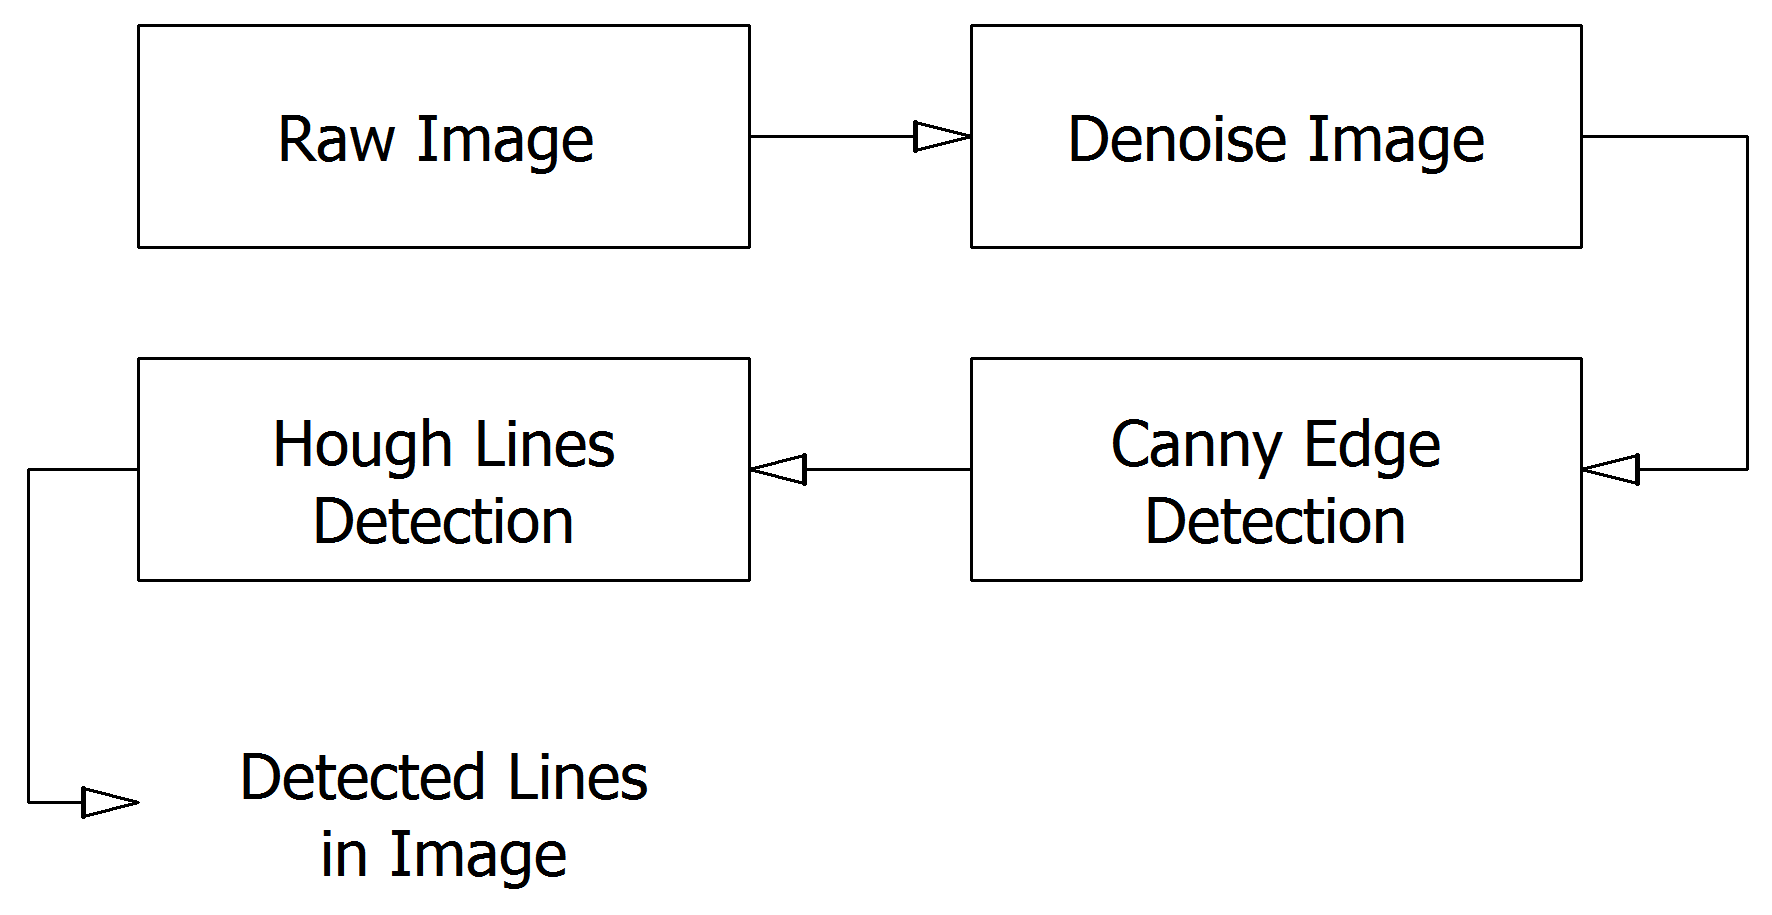
\includegraphics[width=\textwidth]{v-models/lane_detection_subsystem}
\caption{\label{fig:lane_detection_subsystem}The Proposed Algorithm for the Lane Detection.}
\end{figure}
\section{Solutions}

	\subsection{Description of individual sub-systems}

	\subsubsection{Sensing System}

		Sensing system has two main subsystems which are "Lane Detection Subsystem" and "Vehicle Detection Subsystem".
		
		\paragraph{Lane Detection Subsystem}
			The subsystem basically detects the lane. This subsystem uses OpenCV libraries for processing camera frames. The input is captured from a Raspberry Pi camera that is mounted to the vehicle. The captured frame is firstly, preprocessed by a denoising filter. Then, the edges in the frame is detected by Canny Edge Detector algorithm. The output of Canny is a binary image filled with ones and zeros. The Hough Lines technique probabilistically extracts possible lines in a given binary image. Thus, possible line constituting points are obtained from Hough Lines function. Next, points of the lines are classified as left or right borders of the lane. The elimination of the wrong points are done concurrently with the classification. Then, filtered points are fitted in two separate lines to create left and right borders of the lane. As the lane borders are found, the next and the last step is to determine the direction of the vehicle. The output of this subsystem is a turning angle and a direction.

		\paragraph{Vehicle Detection Subsystem}
			The subsystem is the first step of safely computing with an opponent in a racing path. This subsystem uses two laser distance sensors one at the back of the vehicle responsible for detecting the chasing opponent and one at the front of the vehicle responsible for detecting the chased opponent. The subsystem produces positive output if the chasing vehicle or chased vehicle is within a range of 5 cm from the vehicle.			

	\subsubsection{Computation System}
		
		Sensing system has two main subsystems which are "Data Processing Subsystem" and "Controller Subsystem Subsystem".
	
		\paragraph{Data Processing Subsystem}
		
			This unit is the main algorithm application level. Data from sensor will be aggregated in this unit and will be pre-processed. Then, processed data will be output to the controller unit. Processing will mainly be done using Arduino and Raspberry Pi (if used). Suitable algorithms will be developed to realize desired operations with the controller unit

		\paragraph{PID Controller Subsystem}
			
			The output of the data processing subsystem does not mean anything for the vehicle. The motors should be driven using some sort of closed loop system. PID controllers are the most used controller in the robotics field. The purpose of the PID controller is basically to eliminate the error from the desired steady state. In our case the desired steady state  error to be companseted by the


	\subsubsection{Communication System}
	
		Communication system has two main subsystems which are "Internal Communication Subsystem" and "External Communication Subsystem Subsystem".
	
		\paragraph{Internal Communication Subsystem}
		
		\paragraph{External Communication Subsystem}
		
		
	\subsubsection{Driving System}
		
		Driving system has two main subsystems which are "Direction Subsystem" and "Speed Subsystem Subsystem".

		\paragraph{Direction Subsystem}
			Direction unit is responsible for the orientation of the vehicle. It stores the last required orientation and the new one coming from the controller. After that, it tries to make the orientation as close as new one. Both data can be represented as vectors.The angle between those two vector is tried to be minimized by the controller. Before moving on to the operation, note that the angle can be used as a measure of the error that the direction unit have. The less the angle the more correctly operates the direction unit.\\

			
		\paragraph{Speed Subsystem}

		"This unit acts as a complementary module for direction unit. It will act as a state machine. In one state, the unit will try to increase the speed of the vehicle by making overall increase in both PWM values of DC motors. The feedback of this  system will be the cost function mentioned in driving unit. If that cost exceeds a specified level, unit goes to another state in which the unit will decrease the overall speed to allow direction unit to operate more correctly. In short, this unit tries to compensate the error of the direction unit by changing the overall speed of the vehicle.
 

	\subsubsection{Structure System}
	
		Structure system has two main subsystems which are "Chassis Subsystem" and "Printed Circuit Board Subsystem".
		
		\paragraph{Chassis Subsystem}
			Main purposes of this section are protection of the critical elements of the robot and holding components together. The most important part of this section is weight distribution. The chassis is supposed to be light and strong because of the competition purposes. However, it should balance the robot to be able to handle with turns. 
		\paragraph{Printed Circuit Board Subsystem}
			The main role of this part is decreasing connection mass and increase vibration strength of the robot against disturbances. Also, this section increases rigidity of the whole system. 
	
	
	\subsubsection{Motion System}
			
			Motion system has two main subsystems which are "Wheels Subsystem" and "Motors Subsystem Subsystem".		
		
		
		\paragraph{Wheels Subsystem}
			There are possible solution for wheel placement on the chassis, and several wheel types. Some wheels are designed for better gripping on different surfaces. To avoids obstacles on the path, gripping of the wheel is an important concept. Some wheel types are ball caster, toy car wheel and palette. Besides, wheel placement and the wheel number should be combined with the wheel type choice. \\
	
			
		\paragraph{Motors Subsystem}
			Motors are one of the most important physical components of the project. There are possible motor types in the market.\\

			One of the widely used motor type is brushed DC motors. 
			Another option is brushless DC motors. 

			Last option is servo motors.
\subsection{System \& Subsystem Level Requirements}
		
	
	\subsubsection{Sensing System Requirements}
	
		\begin{itemize}
			\item The system should detect the sides of the road.
			\item The system should not be effected from external disturbances.
			\item The system should detect the opponent vehicle.
		\end{itemize}

	\paragraph{Lane Detection Subsystem Requirements}	
		
		\begin{itemize}
			\item The subsystem should be able to detect only the shades of green color
			\item The subsystem should be able to detect edges in the camera frame in any light condition
			\item The subsystem should be able to tell differences between disturbances and lane
			\item The subsystem should be able to interpret the middle of the lane if both sides are present at the frame
		\end{itemize}
	 
	 
	\paragraph{Vehicle Detection Subsystem Requirements}
	
		\begin{itemize}
			\item The subsystem should detect the opponent to be caught with in a 5 cm 
			\item The subsystem should detect the chasing opponent if it reaches from back with in a 5 cm  
		\end{itemize}
		
		
	\subsubsection{Computation System Requirements}
		
		\begin{itemize}
			\item The system should	be able to produce middle line to follow
			\item The system should be able to control the robot
		\end{itemize}			
	
	
	\paragraph{Data Processing Subsystem Requirements}	
	
		\begin{itemize}
			\item The subsystem should be able to analyse data produced by sensing system
			\item The subsystem should be able to produce the angle information required by the controller subsystem
			\item The subsystem should be able to work on Raspberry Pi
			\item The subsystem should be able to process one frame at most in 100 milliseconds
		\end{itemize}
		
	\paragraph{PID Controller Subsystem Requirements}
	
		\begin{itemize}
			\item The subsystem should be able to control the motors
			\item The subsystem should be able to react the external disturbances
		\end{itemize}
	
	\subsubsection{Communication System Requirements}
		
		\begin{itemize}
			\item The subsystem should ensure safe internal communication
			\item The subsystem should ensure safe external communication
		\end{itemize}
	
	\paragraph{Internal Communication Subsystem Requirements}

		\begin{itemize}
			\item The microcontrollers should be able to communicate with each other via serial communication
			\item The internal communication speed should be compatible with the processing speed of the lane detection subsystem  
		\end{itemize}
	
	\paragraph{External Communication Subsystem Requirements}	
	
		\begin{itemize}
			\item The subsystem should be able to communicate with the opponent via Wi-fi protocol
			\item The subsystem should be able to execute handshake protocol
		\end{itemize}
	
	
	\subsubsection{Driving System Requirements}
	
		\begin{itemize}
			\item The subsystem should control motion subsystem according to output of the computation system
		\end{itemize}
	
	\paragraph{Speed Subsystem Requirements}	
		
		\begin{itemize}
			\item The subsystem should decrease the vehicle speed at the narrow lane 
			\item The subsystem should increase the vehicle speed at the wide lane 
			\item The subsystem should decrease the vehicle speed at the extreme disturbance  
		\end{itemize}
		
	\paragraph{Direction Subsystem Requirements}
	
		\begin{itemize}
			\item The subsystem should drive the motors according to computation system outputs
			\item The system should ensure that the vehicle follows the lane 
		\end{itemize}


	\subsubsection{Motion System Requirements}
	
		\begin{itemize}
			\item The system should	ensure that the vehicle can drive itself with enough power
		\end{itemize}
	
	\paragraph{Wheels Subsystem Requirements}	
		
		\begin{itemize}
			\item The subsystem should ensure that the wheels can grip lane without slipping in all conditions 	
		\end{itemize}
		
	\paragraph{Motors Subsystem Requirements}
	
		\begin{itemize}
			\item The subsystem should ensure that the motors can supply enough torque to accelerate the vehicle		
			\item  The subsystem should ensure that the motors can execute driving system outputs without deviation 
		\end{itemize}
	
	
	\subsubsection{Structure System Requirements}
	
		\begin{itemize}
			\item The system should	ensure that structure is robust for external effects 
			\item The system should	ensure that structure is balanced to increase handling
	
		\end{itemize}
	
	\paragraph{Chasis Subsystem Requirements}	
		
			\begin{itemize}
			\item The subsystem should ensure that the chassis is rigid 
			\item The subsystem should ensure that the chassis have enough space for components
			\item The subsystem should ensure that the chassis can provide low center of mass 

		\end{itemize}
		
	\paragraph{PCB Subsystem Requirements}
	
		\begin{itemize}
			\item The subsystem should ensure that all the electronic devices are placed on PCB
			\item The subsystem should ensure that the components are not connected via loose cable 	
		\end{itemize}	



	



	\subsection{Solution for each subsystem and relevant algorithms}
<<<<<<< HEAD
		The applied algorithms, solution steps and solution methodology are presented in this section in a detailed manner.
			\subsubsection{Lane Detection Subsystem}
				The first processing on the captured frame is denoising by blurring. The blurring filter is a GaussianBlur of (3x3) matrix with zero variance both in x and y directions. Next, the filtered image is processed by Canny Edge Detector. This process eliminates all pixels except those are constituting an edge. Edge pixels are usually formed when there is a transition from one object to other. 
				
				Then those detected pixels are input to Hough Lines function. This function outputs two pixels points on the image that form a line. The output of the function is tens of such line points. The accuracy of the function can be adjusted by playing with the input parameters. The function basically draws all lines that might go through a point in the free space (in polar coordinates) and intersects those lines. If the origin points of the intersected lines are within a specified bound, then the line is defined and it can be expanded further. If found points on a line don't exceed a threshold, that line is discarded. The adjustment of such parameters are done with trial and error approach. An important note is that this function is probabilistic, meaning that even if the input frame is never changed, the output line points would be close to previous point but not the same. An example call for this function together with its parameters is given \textit{Script~\ref{sc:hough-call}}.
				
	\begin{lstlisting}[language=C++,float=t,numbers=left,frame=single,caption=Hough Lines Function with its Parameters, captionpos=b, label=sc:hough-call]
HoughLinesP(input=img_threshed, output=line,
	rho=1, theta=CV_PI / 180, threshold=15, 
	minLineLength=30, maxLineGap=40);
	\end{lstlisting}
				Then next step is to classify the line points as left or right. The lines are firstly eliminated according to their slopes. If slope of a line is not in invalid slope region of $\pm$0.005, then it is a valid line. This process is done to get rid of unnecessary low sloped lines. After elimination, line points set must be determined as left or right. At this point, this classification is done according to double checking. the center of the image, that is 320th vertical pixel. If initial and final horizontal points of the image is in the same half, the line belongs to that half. This method works nicely in most regions of the path. However, it is a bit error prone in case of a sharp turning angle or losing one of the lanes . This algorithm will be improved to be more robust.
	\begin{lstlisting}[language=C++,float=t,numbers=left,frame=single,caption=The Algorithm to Classify the Lane Lines as Right or Left, captionpos=b, label=sc:left-right-lines]
std::vector<cv::Vec4i> lines // like a 4x4 matrix
double slope_thresh = 0.005; // absolute threshold slope
for (lines_points) {}
	ini = Point(x1, y1);
	fini = Point(x2, y2);
		line_slope = fini/ini;
	if(abs(line_slope) >= slope_thresh) line_is_valid;
		else line_is_not_valid;

for (lines_is_valid)	
	if(x1>320 && x2>320)
		it_is_right_line;
	else if(x1<320 && x2<320)
		it_is_left_line;
	else discard_the_line;
\end{lstlisting}

			After finding the all left and right line points, actual left and right lines are constructed by applying least square method to the both point sets. The result of this method is 4 points (x1,y1,x2,y2) to refer the left lane line and 4 points to refer the right lane line.
			
			The last process on the image is predicting the turn angle and direction. The prediction of direction is done by comparing the slopes of the left and the right lines. The turning is to be made to the side of the lane line having less slope. The angle is determined by computing the angle between the normal line of the current direction and guide line. Guide line is constructed with the average of the middle points of the right and the left lines and current point of the vehicle. Vehicle's current point is assumed to be in the middle of the beginning of the image. Thus, the beginning point of the guideline is the current position of the vehicle and the endpoint is the target point to be reached. The output of this processing is shown in \textit{Figure~\ref{fig:turn-prediction-explained}}.
				
\begin{figure}[H]
	\center
	\setlength{\unitlength}{\textwidth} 
	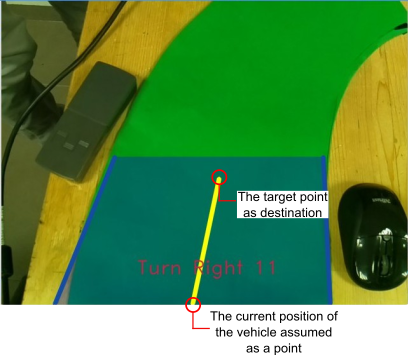
\includegraphics[width=0.6\textwidth]{images/turn-prediction-explained}
	\caption{\label{fig:turn-prediction-explained}The Prediction of Turn Angle and Direction.}
\end{figure}
=======
	
		\subsubsection{Solution for Vehicle Detection Subsystem}
		
			Laser Sensor
	
	
		\subsubsection{Solution for Data Processing Subsystem}
			

		\subsubsection{Solution for Controller Subsystem}
			
			PID Controller
		
		\subsubsection{Solution for Internal Communication Subsystem}
		
			Serial Comm
			
		\subsubsection{Solution for External Communication Subsystem}
		
			Communication subsystem enables the robot to communicate with the opponent using the handshaking. According to the standard committee, Wi-Fi modules must be used to implement handshaking. Since Raspberry Pi was used in the project, there is no need to get a separate Wi-fi module; the internal Wi-fi module of the Raspberry Pi was used. 
			
			Socket programming is an effective tool to implement client-server communication algorithms. It can be implemented in Python or C++.  Our algorithms are written in Python for now, yet it can easily be converted to C++ if the team members decide it is necessary. The algorithms for client and server sides are slightly different. \textit{Figure~\ref{fig:socket_funcs}} shows the functions that are used for client and server sides to create communication between client and server.
			
			
			\begin{figure}[H]
				\center
				\setlength{\unitlength}{\textwidth} 
				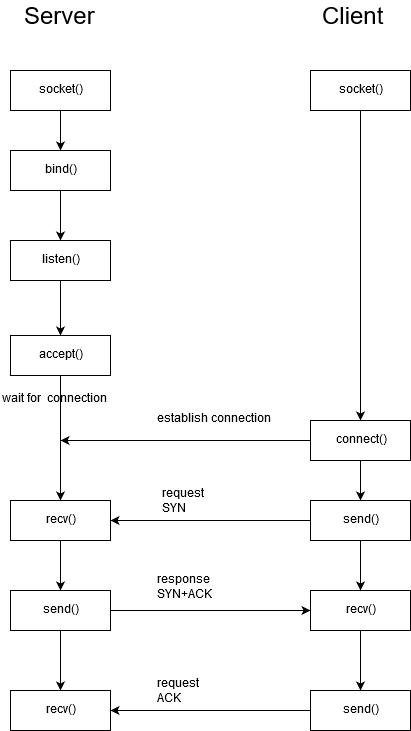
\includegraphics[width=0.55\textwidth]{images/socket_funcs}
				\caption{\label{fig:socket_funcs}TBasic Functions in Python Socket Programming to Implement Handshaking}
			\end{figure}

			Here is the summary of the key functions from socket library:
			
			\begin{itemize}
				\item socket.socket(): Creates a new socket using the given address family, socket type and protocol number.
				\item s.bind(address): Binds the socket to the address defined previously.
      \item s.listen(backlog): Sets up the maximum number of connections that can be made to the socket, which must be at 1 for the project.
\item	s.accept(): Waits until connection arrives, than accept the client connection. Returns the client socket connected to the server as (conn, address) pair, where conn is a new socket object and address is the address bound to this socket
\item	s.connect(): Provides client to connect to the server
\item	s.send(): Transmits message to the remote socket.
\item	s.recv(): Receives message from the remote socket
\item	socket.close(): closes the socket; i.e., ends the communication with the opponent at the end of the race.
			\end{itemize}

			It is stated in the standard committee that each team must be assigned a static IP to communicate with the other robots. Duayenler has the static IP stated as “192.168.1.7” and the ID as “07”. Since Raspberry Pi 3 comes with a built-in wireless adapter, configuring it as a Wi-Fi hotspot is possible. To assign given IP to the robot, Raspberry Pi must be set as an access point from the terminal.
  In the algorithm that was implemented for the handshake, in a continuous loop, the front and rear sensors’ values are been checked. There are two functions which are for client and server modes, respectively. If the front sensor senses the opponent in 5 cm range, our main code visits the client mode function. If the rear sensor senses the opponent in 5 cm range, server mode function runs. If our robot is in the server mode, the rear sensor value is again checked. The acknowledge message(<ID>01) or reject message(<ID>11) is sent according to the sensor value.


		
		\subsubsection{Solution for Direction Subsystem}
		
		
			Depending on the configuration of the wheels, exact control of the vehicle might vary. However, there are certain methods to accomplish orientation. The vehicle will definitely have two wheels or palettes that will be driven by two separate DC motors. That configuration allows differential drive method to orient the vehicle. PWM values of the motors can be adjusted such that the speed difference between them results in a turn as much as desired angle. The exact difference values on the PWM values depends on the specs of the used motors and voltage sources. \\

			Two different H-bridge motor drivers are proposed to be used to drive DC motors: L298N and L293D. Both can drive two motors separately with one IC. However, maximum current rating of the former one is larger being 2A while L293D can supply 0.6A per channel. \\

			
			
		\subsubsection{Solution for Speed Subsystem}

			

		
		\subsubsection{Solution for Chassis Subsystem}
			
			
			
		\subsubsection{Solution for Printed Circuit Board Subsystem}
			
	
		
		\subsubsection{Solution for Wheels Subsystem}
			
	
			One of the possible wheel placement is 2+1 combination. This combination can be assembled by placing 2 car wheels (with motors) to the back and the one boll caster to the front or vice versa. These configurations provide easy implementation and fairly reliable handling on the path. However, for certain obstacles may significantly disturb vehicles balance in this configuration.\\

			
		\subsubsection{Solution for Motors Subsystem}
			
			One of the widely used motor type is brushed DC motors. Such motors might be implemented with gears. Gears are utilized to adjust torque and RPM of the motor, which is very suitable for a racing vehicle's needs. \\

			
	\newpage
	
	
	%%%%%%%%%%%%%%%%%%%%%%%%%%%%%%%%%%	
		
>>>>>>> 4b252a4703aec6dffacf7457c343de22bdf502d3
	\subsection{Subsystem level risk assessment, and alternative solutions (Plan-B)}
	
	
		\subsubsection{Alternative Solutions for Lane Detection Subsystem}
		
			After the module demo result of the camera-oriented lane detection, former solutions are considered to support camera result and enhance robustness of the tracking. Possible future solutions are the followings;  
			
			\paragraph{Laser sensor}
				As IR sensor array solution, which is already considered at the beginning of the term, laser approximate sensors can be constructed as array and used to detect edges of the lane. The expected enhancement is that laser sensors are more robust under extreme illumination conditions. To clarify the solution, two laser sensor arrays sense both sides of the lane. According to array’s data, vehicle orients itself.  


			\paragraph{Color sensor}
				This approach is similar to laser sensor solution, regarding the sensor array construction. However, color sensor working principle is based on RGB recognition, so in this solution green output of the arrays is focused point. According to green output, path will be detected.

	
		\subsubsection{Alternative Solutions for Vehicle Detection Subsystem}
		
			Ultrasonic sensors have acceptable range. They send a sound wave and take back the echo, then give a PWM voltage related to the distance. However, using ultrasonic sensors can cause problems if the opponent also uses ultrasonic sensors; because of the interference. Besides, when measurement is angled, measuring is failing. 

		Infrared sensors can be another approach to this problem, they may provide better accuracy. Moreover, Laser distance measurement can be applied to solve this problem. They have the best accuracy, but their price is the highest among the rest.
	
		\subsubsection{Alternative Solutions for Data Processing Subsystem}
			
		\subsubsection{Alternative Solutions for Controller Subsystem}
			
		
		\subsubsection{Alternative Solutions for Internal Communication Subsystem}
		
		\subsubsection{Alternative Solutions for External Communication Subsystem}
		
		\subsubsection{Alternative Solutions for Direction Subsystem}
		
			As in the case of another configuration that involves one or two servo motors to control the directions of the front wheels. This configuration is more robust compared to ball caster utilization. However, there are more motors to control and it requires more complicated differential drive algorithms involving both DC motor differential and servo PWM to orient the front wheels.
			
			
		\subsubsection{Alternative Solutions for Speed Subsystem}

		
		\subsubsection{Alternative Solutions for Chassis Subsystem}
			
		\subsubsection{Alternative Solutions for Printed Circuit Board Subsystem}
			
	
		
		\subsubsection{Alternative Solutions for Wheels Subsystem}
		
			Another combination is palette system. This system is used in real world where robust vehicles are needed. Similarly, this configuration can help handling obstacle in the path, but it costs for harder implementation and driving.\\

Last implementation is 2+2 configuration. In this configuration 2 wheels can be placed at the back and the rest at the front by placing motors to back wheels. To ease turning of the vehicle, front wheels can be controlled with a servo motor as back wheels operate in the differential drive mode. This combination may provide both enhanced grip and reliable	 operation. \\
			
		\subsubsection{Alternative Solutions for Motors Subsystem}
			
			Another option is brushless DC motors. Brushless DC motors do not use brushes. This results in high torque. Brushless motors are more suitable for high RPM required areas such as CD drivers and drones.\\

			Last option is servo motors. Servo motors are high-torque motors that can turn in an desired angle. Servos can be utilized in the direction of the vehicle on the front wheels. By using this solution, turning radius can be decrease significantly.\\

			
	\newpage
	\subsection{ Error sources, their impact and ways to mitigate}
	
	
	\newpage

	\subsection{System \& Subsystem Tests }


	\subsubsection{Sensing System Tests}

	\paragraph{Lane Detection Subsystem Tests}	
	
		\subparagraph{Light Condition Test}
		
			\begin{itemize}
				\item Mirror the Raspberry Pi screen into Laptop via VNC 
				\item Execute the lane detection algorithm in Raspberry Pi
				\item Change the location of the camera and Pi to conduct test
				\item Observe the results in different locations  
				\item If the visible lane sides can be detected without any additional object, the result of the test can be considered as success.
			\end{itemize}
		
		\subparagraph{Visual Disturbance Test}
		
			\begin{itemize}
				\item Mirror the Raspberry Pi screen into Laptop via VNC 
				\item Execute the lane detection algorithm in Raspberry Pi
				\item Put different objects into lane
				\item Observe the results with different disturbances
				\item If the objects outside of lane is not detected and the objects inside the road only detected only at its border with road, the result of the test can be considered as success.
			\end{itemize}
		
	 
	 
	\paragraph{Vehicle Detection Subsystem Tests}
	
		\subparagraph{•}
		
	\subsubsection{Computation System Tests}
	
	\paragraph{Data Processing Subsystem Tests}	
		
	\paragraph{PID Controller Subsystem Tests}
	
	\subsubsection{Communication System Tests}
	
	\paragraph{External Communication Tests}
	
		The codes that were written in Python were tested in 3 different combinations. The first and simplest test has been done on one computer (or raspberry pi) using the same device as client and server, at the same time. To achieve that, the computer’s (or raspberry pi’s) IP address should be defined in the host section defined in the client mode function. Secondly, the codes were tested on two computers. Thirdly, one raspberry pi and one computer were used for the test. All tests were successful if the server side is connected to the internet and client side is connected to the server via hotspot. The outputs of the tests were given in the \textit{Figure~\ref{fig:handshake1}} and \textit{Figure~\ref{fig:handshake2}}.
		
		
		
		\begin{figure}[H]
				\center
				\setlength{\unitlength}{\textwidth} 
				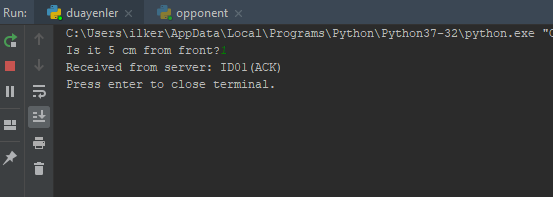
\includegraphics[width=0.75\textwidth]{images/handshake1}
				\caption{\label{fig:handshake1}Test Results of Handshaking for Client Side}
		\end{figure}

		\begin{figure}[H]
			\center
			\setlength{\unitlength}{\textwidth} 
			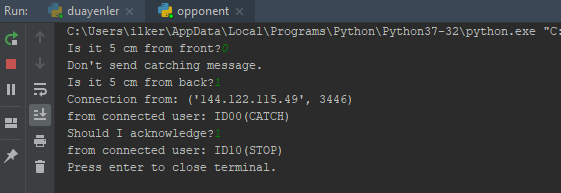
\includegraphics[width=0.75\textwidth]{images/handshake2}
			\caption{\label{fig:handshake2}Test Results of Handshaking for Server Side}
		\end{figure}			
			
	
	\subsubsection{Driving System Tests}
	
	\paragraph{Speed Subsystem Tests}	
		
	\paragraph{Direction Subsystem Tests}


	\subsubsection{Motion System Tests}
	
	\paragraph{Wheels Subsystem Tests}	
		
	\paragraph{Motors Subsystem Tests}
	
	
	\subsubsection{Structure System Tests}
	
	\paragraph{Chasis Subsystem Tests}	
		
	\paragraph{PCB Subsystem Tests}
	
	
	\subsection{Technical drawing of the expected design}
	

\section{Plans}


\section{Conclusion}



\section{Disclaimer}


\end{document}

%----samples------
%\begin{itemize}
%\item Item
%\item Item
%\end{itemize}

%\begin{figure}[H]
%\center
%\setlength{\unitlength}{\textwidth} 
%
\includegraphics[width=0.7\unitlength]{images/logo1}
%\caption{\label{fig:logo}Logo }
%\end{figure}

%\begin{figure}[H]
%	\setlength{\unitlength}{\textwidth} 
%	\centering
%	\begin{subfigure}{.5\textwidth}
%  		\centering
%  		
\includegraphics[width=0.48\unitlength]{images/logo1}
%  		\caption{\label{fig:logo1}Logo1 }
%	\end{subfigure}%
%	\begin{subfigure}{.5\textwidth}
%  		\centering
%		
\includegraphics[width=0.48\unitlength]{images/logo2}
%  		\caption{\label{fig:logo2}Logo2}
%	\end{subfigure}
%\caption{\label{fig:calisandegree} Small Logos   }
%\end{figure}
	
%\begin{table}[H]
%  \centering
% 
%    \begin{tabular}{c|c|c}
%       $$A$$ & $$B$$ & $$C$$ \\ \hline
%       1 & 2 & 3  \\ \hline
%       2 & 3 & 4  \\ \hline
%       3 & 4 & 5  \\ \hline
%       4 & 5 & 6  
%      
%  \end{tabular}
%  \caption{table}
%  \label{tab:table}
%\end{table}
	
%\begin{table}[H]
%  \centering
% 
%    \begin{tabular}{c|c|c}
%       \backslashbox{$A$}{$a$} & $$\specialcell{ Average deviation \\ after subtracting out the  \\ frequency error }$$ & $$C$$ \\ \hline
%       \multirow{2}{*}{1} & 2 & 3  \\ \cline{2-3}
%        & 3 & 4  \\ \hline
%       3 & \multicolumn{2}{c}{4}  \\ \hline
%       4 & 5 & 6  
%      
%  \end{tabular}
%  \caption{table}
%  \label{tab:table}
%\end{table}
%-----end of samples-----